\section*{Arreglos Bidimencionales}

%- - - - - - - - - - - - - - - - - Título - - - - - - - - - - - - - - - - - -%
\begin{frame}[c] 
\centering
\huge \textbf{Arreglos bidimencionales}
\end{frame}

% - - - - - - - - - - - - - - - - - Slide 01 - - - - - - - - - - - - - - - -
\begin{frame}
\frametitle{Arreglos Bidimencionales}
\begin{center}
    \textbf{Definición}
\end{center}
\justify
\hspace{5mm}Un arreglo bidimensional (tabla, matriz) es un conjunto de \textbf{n} elementos del mismo tipo almacenados en una matriz o tabla. A diferencia de los arreglos unidimensionales que sólo requieren de un subíndice, los arreglos bidimensionales para acceder a cada elemento del arreglo requieren de dos índices o subíndices declarados en dos pares de corchetes, donde el primer corchete se refiere al tamaño de filas y el segundo al tamaño de columnas.
\end{frame}


% - - - - - - - - - - - - - - - - - Slide 02 - - - - - - - - - - - - - - - -
\begin{frame}[fragile]
    \frametitle{Arreglos Bidimencionales}
    \begin{center}
        \textbf{Declaración de un arreglo bidimencional}
    \end{center}
    \begin{lstlisting}
    tipoDato identArr[tamFila][tamCol];
    \end{lstlisting}
    Donde:
    \begin{itemize}
        \item \textcolor{blue}{tipoDato} es el tipo de dato de todo el arreglo.\pause
        \item \textcolor{blue}{identArr} es el nombre del arreglo.\pause
        \item \textcolor{blue}{tamFila} es el total de filas.\pause
        \item \textcolor{blue}{tamCol} es el total de columnas.
    \end{itemize}
\end{frame}

% - - - - - - - - - - - - - - - - - Slide 03 - - - - - - - - - - - - - - - -
\begin{frame}[fragile]
    \frametitle{Arreglos Bidimencionales}
    \begin{center}
        \textbf{Ejemplo:\\Declaración de un arreglo de 3 filas y 5 columnas}
    \end{center}
    \begin{lstlisting}
int b[3][5];
\end{lstlisting}
\vspace{-10mm}
\begin{center}
    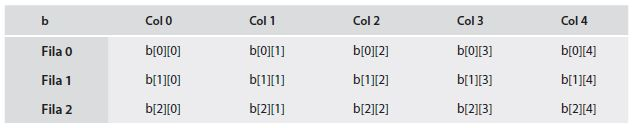
\includegraphics[scale=0.65]{figs/ejemploArregloBidimencional}
\end{center}
\vspace{-6mm}
El número de elementos de una matriz será tamFila 3 tamCol. En el ejemplo anterior son 3 x 5 = 15 celdas de tipo entero.
\end{frame}


% - - - - - - - - - - - - - - - - - Slide 04 - - - - - - - - - - - - - - - -
\begin{frame}[fragile]
    \frametitle{Arreglos Bidimencionales}
    \begin{center}
        \textbf{Inicialización}
    \end{center}
    \vspace{-5mm}
    En el momento de declarar el arreglo, se especifican los valores:
    \begin{lstlisting}
/*tipoDato identif[fil][col] = {valores};*/
int a[3][3] = {1,2,3,4,5,6,7,8,9};
    \end{lstlisting}
    \vspace{-5mm}
    \begin{center}
        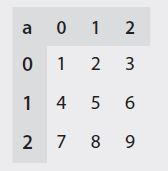
\includegraphics[scale=0.6]{figs/ejemploVisualMatriz}
    \end{center}
\end{frame}

% - - - - - - - - - - - - - - - - - Slide 05 - - - - - - - - - - - - - - - -
\begin{frame}[t, fragile]
    \frametitle{Arreglos Bidimencionales}
    \begin{center}\textbf{Lectura e Impresión}\end{center}
    \justify
    \hspace{5mm}Para la lectura o escritura se requieren de dos ciclos anidados (para ubicar la fila y la columna)en cada celda de la tabla o matriz.
    El siguiente segmento de programa muestra cómo se pueden almacenar datos en una matriz mat de 3
    filas y 4 columnas, se utiliza la instrucción leer (scanf ) para guardar o leer los datos:
    \begin{lstlisting}
for(i=0;i<3;i++)
    for(j=0;j<4;j++)
        scanf("%d", &mat[i][j]);
    \end{lstlisting}
\end{frame}

% - - - - - - - - - - - - - - - - - Slide 06 - - - - - - - - - - - - - - - -
\begin{frame}[fragile]
    \frametitle{Arreglos Bidimencionales}
    El siguiente segmento de programa muestra cómo se pueden imprimir los datos almacenados en una
    matriz mat de 3 filas y 4 columnas. Se utiliza la instrucción imprimir (printf ) para escribir o mostrar el resultado:
    \begin{lstlisting}
for(i=0;i<3;i++)
    for(j=0;j<4;j++)
        printf("%d", mat[i][j]);
    \end{lstlisting}
\end{frame}

% - - - - - - - - - - - - - - - - - Slide 07 - - - - - - - - - - - - - - - -
\begin{frame}[fragile]
    \frametitle{Arreglos Bidimencionales}
    \begin{center}
        \textbf{Modificación de un elemento de un arreglo Bidimencional}
    \end{center}
    Los elementos de un arreglo bidimencional se pueden modificar en cualquier momento, sólo es necesario especificar el nombre del arreglo bidimensional, la posición tanto de la fila como de la columna y el nuevo valor. En seguida se muestra la sintaxis a seguir:
    \begin{lstlisting}
identArr [fil][col] = valor;
    \end{lstlisting}
    Donde valor es un dato o el resultado de alguna operación lógica o aritmética, etc.
    \begin{lstlisting}

    \end{lstlisting}
\end{frame}